% ACM Computing Surveys-style student review manuscript
% Converted from the supplied manuscript. Content is preserved; changes are limited
% to LaTeX structure, cross-referencing, citation mechanics, and standard metric equations.
\documentclass[acmsmall]{acmart}

\setcopyright{none}
\settopmatter{printacmref=false}
\renewcommand\footnotetextcopyrightpermission[1]{}
\acmJournal{CSUR}
\citestyle{acmauthoryear}

% Packages needed for the preserved figures/table and standard metric equations.
\usepackage{graphicx}
\usepackage{booktabs}
\usepackage{tabularx}
\usepackage{stfloats}
\usepackage{array}
\usepackage{amsmath}
%\usepackage{placeins}

% Allow the full-width literature table to fit near its first citation without drifting to the references.
\renewcommand{\dbltopfraction}{0.95}
\renewcommand{\dblfloatpagefraction}{0.85}
\setcounter{dbltopnumber}{1}

% Author information was not present in the supplied manuscript.
% Replace the placeholder block before submission.
\author{Author Name}
\affiliation{%
  \institution{Institution Name}
  \city{City}
  \country{Country}
}

\title{Evaluating Tool-Selection Accuracy in Multi-Tool Agentic AI Systems}
\subtitle{A Survey of Metrics, Benchmarks, and Open Challenges}

\begin{abstract}
As large language models (LLMs) are increasingly deployed as autonomous agents that must choose among many external functions, application programming interfaces (APIs), and plug-ins to satisfy a user instruction, the accuracy with which an agent selects the correct tool from a candidate set has emerged as a central determinant of end-to-end task success. This paper surveys the evaluation of tool-selection accuracy in multi-tool agentic systems. We synthesize a taxonomy of the sub-problems involved --- invocation necessity detection, tool discrimination among semantically overlapping candidates, tool retrieval from large repositories, argument grounding, and multi-step trajectory ordering --- and review the metrics (exact-match accuracy, F1 over predicted tool sets, mean reciprocal rank, pass rate, and trajectory-level diagnostics) that the literature uses to quantify each. We examine current benchmarking efforts, including ToolLLM/ToolBench, API-Bank, MetaTool, TaskBench, the Berkeley Function-Calling Leaderboard, and recent trajectory-aware suites, and compare how they operationalize tool-selection accuracy differently. We then discuss recurring failure modes reported across this literature, including confusion among functionally similar tools, degraded selection accuracy as candidate-set size grows, sensitivity to tool-description phrasing, and the difficulty of evaluating tool selection independently of downstream execution correctness. Finally, we identify gaps --- particularly around standardized cross-benchmark metrics, evaluation of tool selection under dynamic or evolving tool sets, and multi-agent tool-sharing scenarios --- and outline directions for future research. The review is intended to give researchers and practitioners a consolidated reference point for designing and interpreting tool-selection evaluations in agentic AI systems.
\end{abstract}

\keywords{tool selection, agentic AI, large language models, function calling, tool retrieval, benchmark evaluation, API selection, autonomous agents}

\ccsdesc[500]{Computing methodologies~Natural language processing}
\ccsdesc[300]{Computing methodologies~Machine learning approaches}
\ccsdesc[200]{Information systems~Information retrieval}

\begin{document}
\maketitle

\section{Introduction}
\label{sec:introduction}

Large language models (LLMs) have moved beyond single-turn text generation into agentic configurations in which a model plans, acts, and observes the results of actions taken through external tools --- search engines, calculators, databases, code interpreters, and arbitrary third-party APIs \citep{yao2023react,schick2023toolformer}. This shift is often summarized as ``tool use'' or ``tool learning,'' and it has been identified as one of the defining capabilities that separate a conversational LLM from an autonomous agent capable of completing multi-step real-world tasks \citep{qu2025survey}. As the number of tools exposed to an agent grows --- from a handful of hand-written functions to repositories containing thousands of real-world RESTful APIs \citep{qin2024toolllm,patil2023gorilla} --- the agent's ability to identify which tool, among many plausible candidates, is appropriate for a given sub-task becomes a first-order bottleneck on system reliability.

Tool-selection accuracy refers to whether an agent chooses the correct tool (or correct set of tools) from a defined or retrieved candidate list to address a given user request or sub-task, prior to and independent of whether the agent supplies correct arguments or achieves a correct final outcome \citep{mohammadi2025evaluation}. This is distinct from, but closely coupled to, the broader notion of tool-use accuracy, which additionally requires correct parameterization and successful execution \citep{shen2023taskbench,li2023apibank}. In practice, tool-selection errors compound: an agent that calls the wrong weather API will not produce a correct answer no matter how well it formats the request, and an agent that fails to recognize that a tool is needed at all will hallucinate an answer instead of retrieving one \citep{huang2024metatool}.

The problem is non-trivial for several reasons. First, real-world tool repositories frequently contain multiple tools with overlapping or near-duplicate functionality, which forces the agent to discriminate on the basis of subtle differences in documented behavior, input schema, or scope \citep{qin2024toolllm}. Second, as the size of the tool set grows beyond what can be placed in a prompt context window, tool selection becomes entangled with information retrieval: the agent, or a retriever acting on its behalf, must first narrow thousands of candidates down to a shortlist before a final selection can be made, introducing a second source of error upstream of the LLM's own reasoning \citep{shi2025toolretrieval}. Third, many realistic tasks require selecting and sequencing multiple tools, so that selection accuracy must be evaluated not as an isolated classification decision but as part of a trajectory whose correctness depends on order and dependency structure \citep{shen2023taskbench}.

This paper reviews how the research community defines, measures, and benchmarks tool-selection accuracy in multi-tool agentic AI systems. We organize the discussion around four questions: (1) What sub-problems constitute ``tool selection,'' and how are they distinguished in the literature? (2) What metrics have been proposed to quantify tool-selection accuracy, and what do they capture or omit? (3) What benchmarks and current systems exist, and how do their design choices affect the comparability of reported results? (4) What methodological gaps and open research questions remain? The remainder of the paper is organized as follows. Section~\ref{sec:background} reviews background and related work on tool-augmented LLMs and agent evaluation. Section~\ref{sec:technical} presents a technical discussion of tool-selection accuracy, its constituent sub-tasks, and associated metrics. Section~\ref{sec:approaches} surveys current approaches, systems, and benchmarks. Section~\ref{sec:challenges} discusses limitations and challenges reported in the literature. Section~\ref{sec:gaps} identifies research gaps and future directions, and Section~\ref{sec:conclusion} concludes.

\section{Background and Related Work}
\label{sec:background}

Tool-augmented language modeling has its roots in efforts to overcome LLMs' known weaknesses in precise computation, up-to-date factual retrieval, and interaction with external systems. Toolformer demonstrated that a language model could be trained, in a largely self-supervised manner, to decide when to invoke an API, which API to invoke, and how to incorporate its output into subsequent generation, using a small set of tools including a calculator, a question-answering system, and a calendar \citep{schick2023toolformer}. Around the same period, ReAct proposed interleaving explicit reasoning traces with discrete actions, allowing a model to update its plan in light of intermediate observations from tools or environments rather than committing to a single upfront plan \citep{yao2023react}. These two lines of work established the now-standard ``think--act--observe'' loop that underlies most contemporary agent architectures \citep{schick2023toolformer,yao2023react}.

A second wave of work scaled the number and diversity of available tools. Gorilla fine-tuned a LLaMA-based model with retrieval-aware training so that it could generate accurate API calls against a large, evolving set of machine learning framework APIs, and showed that a fine-tuned smaller model could outperform GPT-4 on this task when equipped with an appropriate retriever \citep{patil2023gorilla}. ToolLLM extended this idea to general-purpose, real-world RESTful APIs at much larger scale, constructing ToolBench from 16,464 APIs spanning 49 categories collected from the RapidAPI Hub, and introducing a depth-first search-based decision tree algorithm to allow an LLM to explore and backtrack across multiple reasoning traces during tool use \citep{qin2024toolllm}. HuggingGPT took a complementary approach, using an LLM as a controller that decomposes a task and dispatches sub-tasks to specialized models hosted on the Hugging Face platform, effectively treating other models as tools \citep{shen2023hugginggpt}.

Figure~\ref{fig:tool-scale} visualizes the growth in tool-repository scale across the benchmarks introduced above.

\begin{figure*}[t]
  \centering
  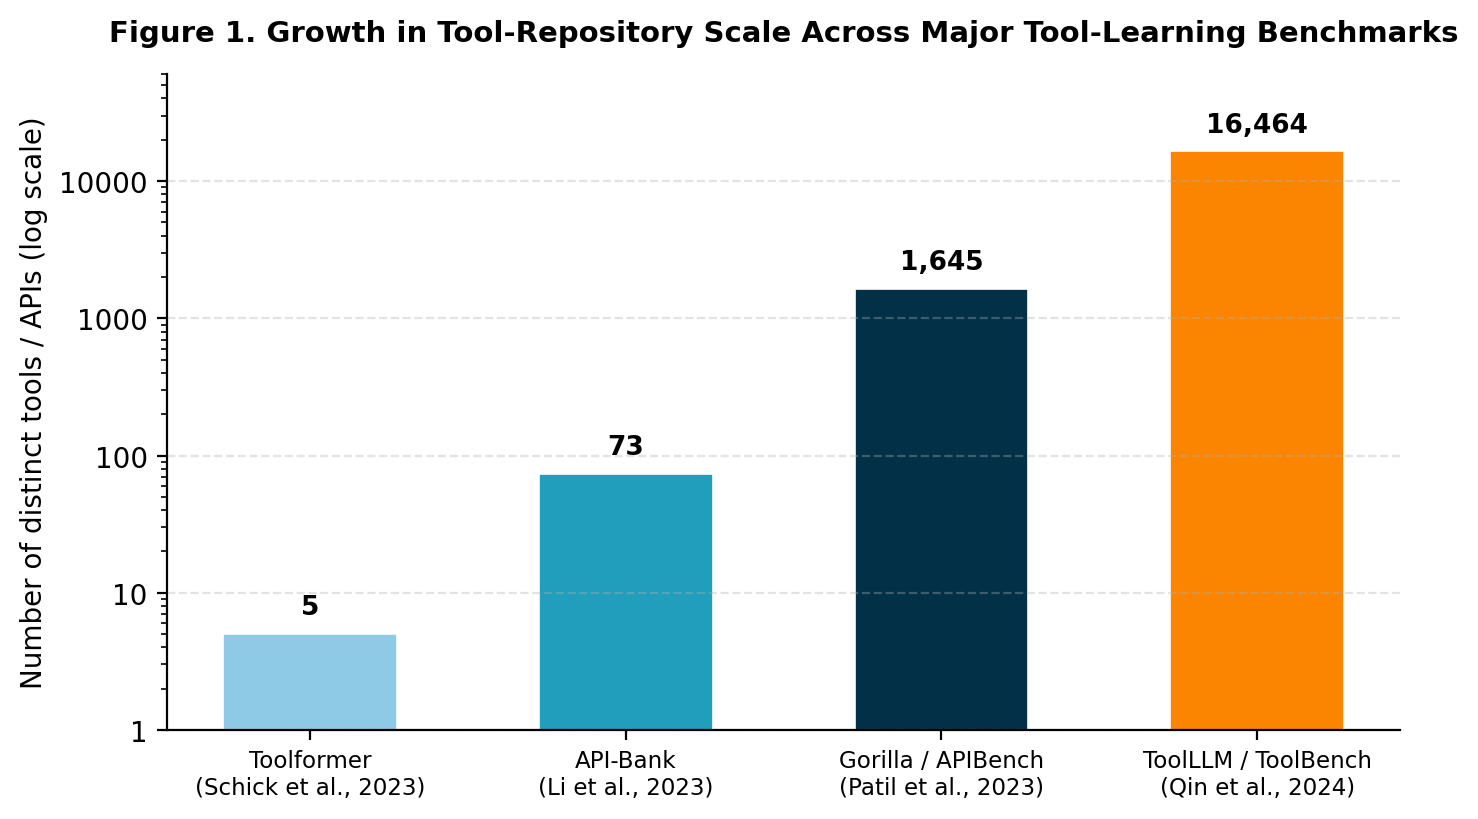
\includegraphics[width=0.88\textwidth]{figures/tool_repository_scale.png}
  \caption{Growth in Tool-Repository Scale Across Major Tool-Learning Benchmarks (log scale).}
  \label{fig:tool-scale}
  \Description{A logarithmic bar chart comparing tool-repository scale for Toolformer, API-Bank, Gorilla/APIBench, and ToolLLM/ToolBench.}
  \par\smallskip
  \footnotesize Sources: \citet{schick2023toolformer}; \citet{li2023apibank}; \citet{patil2023gorilla}; \citet{qin2024toolllm}.
\end{figure*}

Table~\ref{tab:comparison} consolidates the studies discussed above into a single comparative matrix spanning methodology, evaluation scale, metrics, key findings, and limitations.

\begin{table*}[!t]
  \centering
  \caption{Comprehensive Literature and Method Comparison Matrix}
  \label{tab:comparison}
  \setlength{\tabcolsep}{2pt}
  \renewcommand{\arraystretch}{0.82}
  \scriptsize
  \begin{tabularx}{\textwidth}{@{}>{\raggedright\arraybackslash}X>{\raggedright\arraybackslash}X>{\raggedright\arraybackslash}X>{\raggedright\arraybackslash}X>{\raggedright\arraybackslash}X>{\raggedright\arraybackslash}X@{}}
    \toprule
    \textbf{Study (Year)} & \textbf{Method / Approach} & \textbf{Tool-Repository / Sample Scale} & \textbf{Evaluation Metric(s)} & \textbf{Key Finding} & \textbf{Principal Limitation} \\
    \midrule
    \textbf{Schick et al. (2023) Toolformer} & Self-supervised API-call insertion into LM pretraining & 5 tools (QA, calculator, search, calendar, MT) & Task-specific zero-/few-shot accuracy & Small LM + tool calls can match/exceed larger LMs on select tasks & Tool set too small to stress-test selection among many candidates \\
    \textbf{Yao et al. (2023) ReAct} & Interleaved reasoning traces + discrete actions & Task-dependent (QA, ALFWorld, WebShop) & Task success rate; reasoning-trace quality & Reasoning improves action/tool choice vs.\ acting-only baselines & No explicit isolation of selection error from planning error \\
    \textbf{Patil et al. (2023) Gorilla / APIBench} & Retriever-aware fine-tuning (RAT) of LLaMA & 1,645 unique APIs; 16,450 instruction pairs & AST tree exact-match accuracy & Fine-tuned 7B model outperforms GPT-4 on API call generation & Generalization tested mainly within ML-framework API domain \\
    \textbf{Li et al. (2023) API-Bank} & Runnable multi-turn dialogue evaluation system & 73 APIs; several hundred annotated dialogues & API-call correctness; retrieval + planning accuracy & Separates tool retrieval from tool-call correctness for the first time at scale & Tool set size modest relative to later benchmarks \\
    \textbf{Shen et al. (2023) HuggingGPT} & LLM controller dispatches sub-tasks to expert models & $\sim$20+ Hugging Face expert models as ``tools'' & Task completion via model-selection success & Treating other models as tools generalizes across modalities & Latency and cascading-error risk across chained model calls \\
    \textbf{Qin et al. (2024) ToolLLM / ToolBench} & DFS-based decision tree + neural API retriever & 16,464 real-world APIs; 49 categories & Pass rate; win rate (vs.\ reference solution) & DFS exploration improves multi-step tool-use success over single-chain reasoning & Reliance on API-call simulation for unavailable live APIs \\
    \textbf{Huang et al. (2024) MetaTool} & ToolE dataset spanning 4 selection subtasks & 4,287 test instances; 199 tools & Selection accuracy; reliability (no-tool) accuracy & Majority of 8 tested LLMs struggle on similar-tool and reliability subtasks & English-only prompts; synthetic query generation \\
    \textbf{Shen et al. (2023) TaskBench} & Tool-graph construction (nodes + dependency edges) & 3 domains; multiple tool/task graphs & Node-F1; Edge-F1; Normalized Edit Distance & Sequencing errors are distinct from and additive to pure selection errors & Graph-construction annotation is costly to scale to new domains \\
    \textbf{Patil et al. (2025) BFCL (v1--v4)} & Deterministic AST matching vs.\ reference call & Thousands of function-call test cases, multi-turn & AST exact-match rate & Standardized, reproducible leaderboard enables cross-model comparison over time & AST match conflates wrong-tool and wrong-argument errors \\
    \textbf{Shi et al. (2025) Tool-retrieval study} & Benchmarking dense/sparse retrievers for tools & Multiple tool-retrieval benchmarks (ACL Findings) & Recall@k; Mean Reciprocal Rank & General-purpose text retrievers under-retrieve functionally correct tools & Findings limited to text-embedding retrievers evaluated at time of study \\
    \textbf{Qian et al. (2025) ToolRL} & RL reward design for tool-integrated reasoning & Multiple tool-use RL training environments & Task success under RL reward; generalization to unseen tools & Reward-driven training improves generalization vs.\ supervised fine-tuning alone & Reward design remains heuristic; not selection-specific by default \\
    \textbf{Wang et al. (2024) MTU-Bench} & Multi-granularity dialogue synthesis via GPT-4 & 54,798 dialogues; 136 tools & Tool-selection accuracy; tool-order accuracy; task-process rate & Fine-grained metrics reveal separate order- vs.\ selection-error sources & Synthetic data generation introduces GPT-4-specific annotation bias \\
    \textbf{He et al. (2025) TRAJECT-Bench} & Trajectory-level diagnostic decomposition & Multi-hop, multi-tool trajectories & Selection, argument, and order/dependency scores (reported separately) & ``Similar-tool confusion'' and ``parameter-blind selection'' are dominant error modes & Diagnostic granularity not yet adopted by most other benchmarks \\
    \bottomrule
  \end{tabularx}

  \par\smallskip
  \footnotesize Sources: \citet{schick2023toolformer}; \citet{yao2023react}; \citet{patil2023gorilla}; \citet{li2023apibank}; \citet{shen2023hugginggpt}; \citet{qin2024toolllm}; \citet{huang2024metatool}; \citet{shen2023taskbench}; \citet{patil2025bfcl}; \citet{shi2025toolretrieval}; \citet{qian2025toolrl}; \citet{wang2024mtubench} (MTU-Bench); \citet{he2025trajectbench} (TRAJECT-Bench).
\end{table*}

In parallel, a distinct benchmarking literature emerged to evaluate these systems. API-Bank annotated several hundred multi-turn, tool-use dialogues against a runnable evaluation system of 73 APIs, explicitly separating an agent's ability to call a given API from its ability to first retrieve the correct API and plan a sequence of calls \citep{li2023apibank}. MetaTool went further by directly targeting the selection decision, introducing the ToolE dataset of user queries annotated for whether a tool is needed at all and, if so, which single tool or combination of tools is appropriate, including deliberately confusable groups of tools with overlapping functionality \citep{huang2024metatool}. TaskBench reframed tool selection as a graph-construction problem, in which an agent must correctly identify the nodes (tools) and edges (dependencies) of a task-specific ``tool graph,'' and proposed Node-F1 and Edge-F1 metrics that separately credit correct tool identification and correct sequencing \citep{shen2023taskbench}. The Berkeley Function-Calling Leaderboard (BFCL) subsequently standardized evaluation of native function-calling APIs offered by commercial and open-source model providers, using deterministic abstract-syntax-tree (AST) matching against reference function calls across single-turn, multi-turn, and, in its most recent iteration, broader agentic scenarios \citep{patil2025bfcl}.

\citet{qu2025survey} organize the tool-learning literature around a four-stage workflow --- task planning, tool selection, tool calling, and response generation --- and catalog the benefits tool integration provides, from expanding an LLM's effective knowledge boundary to improving interpretability of its outputs. A broader survey of LLM agent evaluation similarly distinguishes tool-selection accuracy, defined as choosing the correct tool from a list of options, from retrieval accuracy, defined as identifying the correct tool from a larger repository via natural-language matching, treating the two as related but separable evaluation targets \citep{mohammadi2025evaluation}. This distinction between selection from a small, given candidate set and retrieval from a large, open-ended repository recurs throughout the literature reviewed in this paper and motivates the taxonomy presented in Section~\ref{sec:decompose}.

Table~\ref{tab:comparison} consolidates the studies discussed above into a single comparative matrix spanning methodology, evaluation scale, metrics, key findings, and limitations.


\section{Tool-Selection Accuracy: A Technical Discussion}
\label{sec:technical}

\subsection{Decomposing the Tool-Selection Problem}
\label{sec:decompose}

The literature converges on decomposing an agent's overall tool-use competence into a small number of sequential sub-decisions, each of which can fail independently and each of which has been assigned distinct evaluation protocols \citep{mohammadi2025evaluation,qu2025survey}:

\begin{itemize}
  \item \textbf{Invocation necessity detection:} deciding whether any external tool is required at all, as opposed to answering directly from parametric knowledge. MetaTool's ToolE dataset explicitly includes queries for which no tool is appropriate, to measure over-triggering as well as under-triggering \citep{huang2024metatool}.
  \item \textbf{Tool discrimination (selection proper):} given a fixed, enumerated candidate set --- often deliberately containing functionally similar or overlapping tools --- choosing the single tool or subset of tools that correctly matches the request \citep{huang2024metatool,qin2024toolllm}.
  \item \textbf{Tool retrieval:} when the full candidate set is too large to place in context, first narrowing a repository of hundreds or thousands of tools to a shortlist using dense or sparse retrieval over natural-language tool descriptions, a step whose errors are attributable to the retriever rather than the LLM's reasoning \citep{shi2025toolretrieval,qin2024toolllm}.
  \item \textbf{Argument grounding:} once a tool is selected, generating correct and complete input parameters; commonly evaluated jointly with, but conceptually distinct from, selection \citep{patil2023gorilla,patil2025bfcl}.
  \item \textbf{Trajectory-level selection and ordering:} in multi-hop tasks, correctly selecting a sequence of interdependent tools and respecting their data-flow and ordering constraints, evaluated with graph- or trajectory-level metrics rather than single-decision accuracy \citep{shen2023taskbench,he2025trajectbench}.
\end{itemize}

Figure~\ref{fig:pipeline} depicts these five sub-decisions as a single end-to-end pipeline.

\begin{figure*}[t]
  \centering
  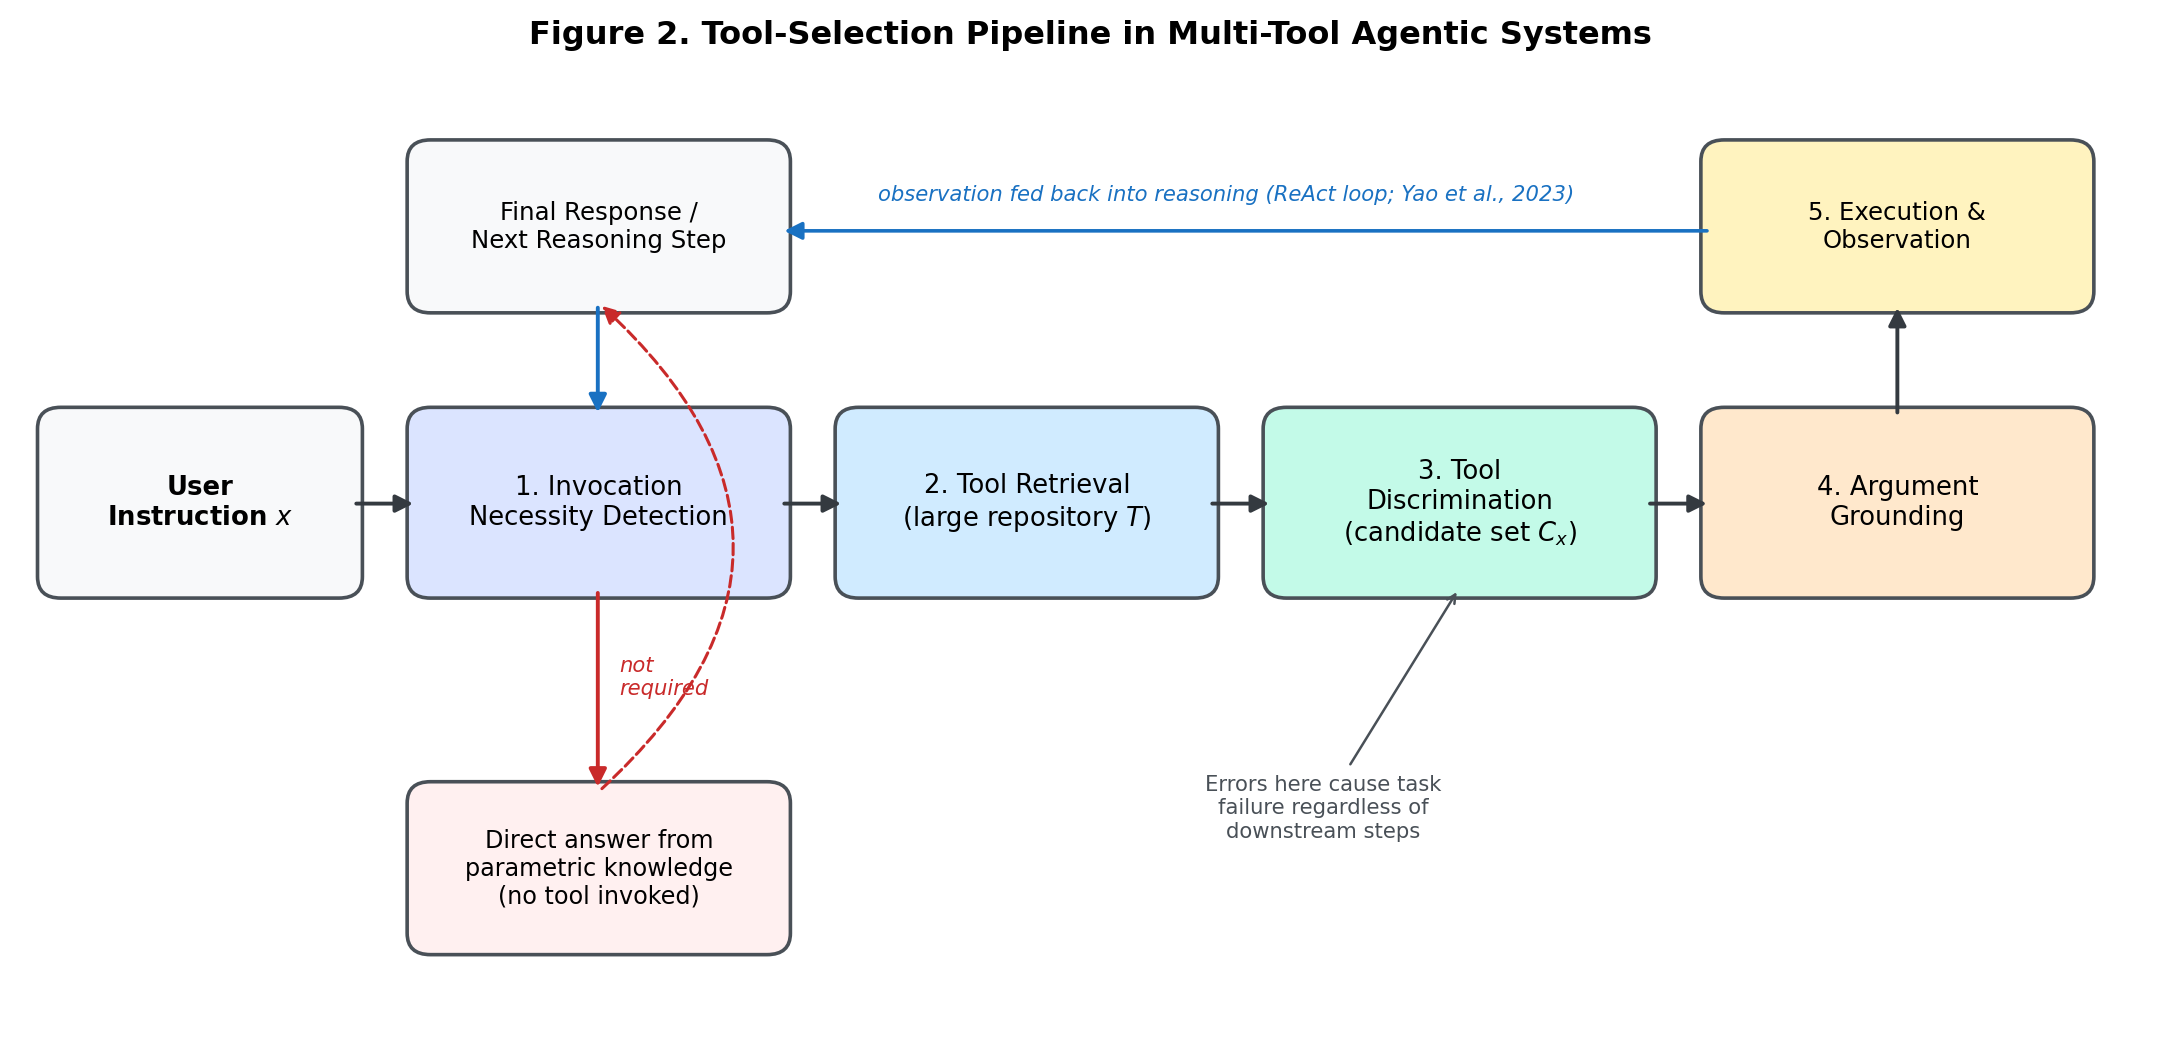
\includegraphics[width=0.97\textwidth]{figures/tool_selection_pipeline.png}
  \caption{Tool-Selection Pipeline in Multi-Tool Agentic Systems.}
  \label{fig:pipeline}
  \Description{A pipeline diagram showing invocation necessity detection, tool retrieval, tool discrimination, argument grounding, execution and observation, and feedback to the next reasoning step.}
  \par\smallskip
  \footnotesize Sources: \citet{yao2023react}; \citet{huang2024metatool}; \citet{qin2024toolllm}; \citet{shi2025toolretrieval}; \citet{shen2023taskbench}.
\end{figure*}

\subsection{Metrics}
\label{sec:metrics}

Because the sub-problems above differ structurally, the metrics applied to them differ as well. At the simplest level, exact-match or top-1 accuracy over a closed candidate set is used when a query maps to exactly one correct tool, as in MetaTool's single-tool setting \citep{huang2024metatool} and in several ablations of MLLM-Tool, which reports 88.19\% tool-selection accuracy after fine-tuning on its multimodal ToolMMBench benchmark \citep{wang2025mllmtool}. When a query may legitimately require zero, one, or several tools simultaneously, set-based metrics such as precision, recall, and F1 over the predicted tool set are preferred, since accuracy alone penalizes partially correct multi-tool predictions too harshly \citep{huang2024metatool}.

For the standard set-based F1 definition, with precision $P$ and recall $R$:
\begin{equation}
F_1 = \frac{2PR}{P+R}.
\label{eq:f1}
\end{equation}
Thus, the F1 definition referred to in this section is given in Eq.~\eqref{eq:f1}.

For the retrieval stage, where the goal is to surface the correct tool within a ranked shortlist rather than to name it outright, rank-based metrics such as Recall@k and Mean Reciprocal Rank (MRR) are standard, mirroring their use in information retrieval more broadly \citep{mohammadi2025evaluation,shi2025toolretrieval}. The MRR definition used for a set of $N$ queries, with $\operatorname{rank}_i$ denoting the rank of the first relevant tool for query $i$, is:
\begin{equation}
\mathrm{MRR} = \frac{1}{N}\sum_{i=1}^{N}\frac{1}{\operatorname{rank}_i}.
\label{eq:mrr}
\end{equation}
The MRR definition is therefore given in Eq.~\eqref{eq:mrr}. For trajectory- or graph-structured tasks, TaskBench introduces Node-F1 to score tool identification independent of order, Edge-F1 to score correctly predicted dependencies between tools, and a Normalized Edit Distance (NED) to specifically penalize incorrect sequencing in chain-structured tasks \citep{shen2023taskbench}. More recent trajectory-aware benchmarks extend this by reporting tool-selection and argument correctness alongside separate dependency- and order-satisfaction diagnostics, explicitly aiming to avoid collapsing several distinct failure modes into a single pass/fail outcome \citep{he2025trajectbench}.

Finally, function-calling leaderboards such as BFCL evaluate selection indirectly through deterministic Abstract Syntax Tree (AST) comparison between a model's generated function call and a reference call, which implicitly scores whether the correct function name was chosen as part of a broader exact-match criterion that also covers arguments \citep{patil2025bfcl}. This approach trades some diagnostic granularity --- it does not by default separate ``wrong function'' from ``right function, wrong argument'' errors in the headline score --- for reproducibility and freedom from the cost and variance associated with LLM-as-judge evaluation \citep{patil2025bfcl}.

\subsection{Candidate-Set Composition and Task Design}
\label{sec:candidates}

A recurring methodological theme is that reported tool-selection accuracy is highly sensitive to how the candidate tool set is constructed. Benchmarks that include ``confusable'' groups of tools with similar names or overlapping descriptions, as MetaTool does by design, produce systematically lower accuracy than benchmarks whose candidate tools are more clearly differentiated \citep{huang2024metatool}. Similarly, MLLM-Tool's analysis found that when multiple API options exist for a query, the difficulty of correctly discriminating among them depends heavily on the ambiguity category of the query, with certain ambiguity types (e.g., differences in quality or operating conditions) yielding markedly higher selection accuracy than others \citep{wang2025mllmtool}. These findings imply that tool-selection accuracy figures are not directly comparable across benchmarks unless the composition and difficulty of the candidate set are controlled for or reported alongside the headline number.

\section{Current Approaches and Developments}
\label{sec:approaches}

\subsection{Prompting- and Reasoning-Based Approaches}
\label{sec:prompting}

The dominant paradigm for eliciting tool selection from general-purpose LLMs remains prompting the model with a list of available tools (typically as structured schemas) and relying on in-context reasoning to select and parameterize the appropriate one, following the interleaved reasoning-and-acting pattern established by ReAct \citep{yao2023react}. Systems such as HuggingGPT extend this by having the controller LLM select not only atomic API calls but entire downstream expert models based on natural-language task descriptions \citep{shen2023hugginggpt}. AutoTool and related work explore reducing the cost of this reasoning loop by more efficiently pruning the candidate space before invoking the LLM's full reasoning capability, reporting evaluation across multi-hop benchmarks including ALFWorld, ScienceWorld, and academic API-query tasks \citep{jia2025autotool}.

\subsection{Fine-Tuning and Retrieval-Augmented Selection}
\label{sec:retrieval}

A second line of work fine-tunes models specifically for tool selection and invocation, rather than relying solely on prompting. Gorilla's retriever-aware training (RAT) couples a document retriever with fine-tuning so that the model can adapt to test-time changes in API documentation, such as version or argument updates, rather than memorizing a fixed API surface \citep{patil2023gorilla}. ToolLLM similarly fine-tunes an open-source LLaMA-based model on ToolBench-derived trajectories, augmented with a neural API retriever and a depth-first search-based decision-making algorithm that allows exploration of multiple candidate tool sequences before committing to one \citep{qin2024toolllm}. Because a fixed context window cannot accommodate documentation for thousands of tools simultaneously, retrieval-augmented tool selection --- dense or sparse retrieval over tool descriptions to produce a shortlist prior to LLM-based selection --- has become a near-universal architectural component in large-scale tool-use systems, though recent work cautions that standard text retrievers are not inherently ``tool-savvy'' and can systematically under-retrieve functionally correct but lexically dissimilar tools \citep{shi2025toolretrieval}.

\subsection{Reinforcement Learning for Tool Use}
\label{sec:rl}

Most recently, reinforcement-learning-based post-training has been applied to tool selection and broader tool-integrated reasoning, using reward signals derived from whether the correct tool was called and whether the resulting trajectory achieved the task outcome, rather than relying solely on supervised imitation of annotated trajectories. ToolRL, for example, proposes reward design specifically for tool-use learning and reports that reward-driven training can improve generalization to unseen tools relative to supervised fine-tuning alone \citep{qian2025toolrl}. This reflects a broader shift in the field toward treating correct tool selection as an outcome to be optimized directly, in addition to being an evaluation target measured post hoc.

\subsection{Standardized Benchmarking Infrastructure}
\label{sec:benchmarking}

On the evaluation side, the field has moved toward standardized, versioned leaderboards rather than one-off benchmark papers. BFCL has iterated through multiple versions, progressively adding enterprise- and community-contributed functions, multi-turn interaction evaluation, and, in its fourth version, a more holistic agentic evaluation that extends beyond isolated function calls \citep{patil2025bfcl}. Complementing this, multi-granularity benchmarks such as MTU-Bench aim to evaluate tool use across single-tool, multi-tool, and multi-turn settings within a unified framework, and multi-agent-oriented benchmarks such as Tool-RoCo extend the notion of ``tool'' to include other cooperating agents, revealing that current LLM-based agents rarely invoke one another as assistants even when a cooperative-tool option is available \citep{wang2024mtubench,zhang2025toolroco}.

\section{Research Challenges and Limitations}
\label{sec:challenges}

Several challenges recur across the literature reviewed above. First, similar-tool confusion remains a persistent failure mode: models struggle to discriminate between tools with overlapping functionality or similar names, and this confusion is often the dominant error source in benchmarks specifically designed to probe it \citep{huang2024metatool}. A recent trajectory-aware evaluation similarly identifies ``similar tool confusion'' and ``parameter-blind selection'' as recurring failure patterns, and further finds that models struggle disproportionately to infer the correct tool from queries that describe a need indirectly rather than naming the required capability explicitly \citep{he2025trajectbench}.

Second, selection accuracy degrades as the candidate or repository size grows. Once the number of available tools exceeds what can be enumerated in context, systems must rely on a retrieval stage whose own errors are compounded with the LLM's selection errors, and current dense or sparse retrievers have been shown to be imperfectly suited to the tool-retrieval task specifically, as opposed to generic semantic-similarity retrieval, in part because textual similarity between a query and a tool description does not always track functional correctness \citep{shi2025toolretrieval}.

Third, evaluation itself is methodologically inconsistent across the field. Different benchmarks use different unit-of-analysis choices --- single-decision accuracy, set-based F1, ranked retrieval metrics, or graph-based node/edge scores --- making it difficult to compare reported tool-selection accuracy figures across papers without re-implementing evaluation protocols \citep{shen2023taskbench,mohammadi2025evaluation}. Benchmarks that rely on LLM-as-judge scoring, as opposed to deterministic matching such as BFCL's AST comparison, introduce additional variance and cost, and their judgments may not be fully reproducible across model versions \citep{patil2025bfcl}.

Fourth, most existing evaluations assume a largely static, well-documented tool set known in advance. Real deployments, by contrast, may involve tools whose documentation, arguments, or availability change over time, or whose descriptions are noisy, incomplete, or adversarially misleading; Gorilla's retriever-aware training was motivated specifically by the observation that standard fine-tuning does not generalize well to such test-time API changes \citep{patil2023gorilla}. Multi-robot and multi-agent settings introduce a further complication, since ``tools'' in these settings can themselves be other autonomous agents with their own state, and current systems have been shown to rarely make effective use of cooperative-tool options even when they would improve task outcomes \citep{zhang2025toolroco}.

Finally, tool selection is difficult to evaluate in isolation from downstream execution. Because a wrong tool selection typically causes a cascading task failure, many end-to-end benchmarks report only an aggregate task-success or progress-rate metric, from which the specific contribution of selection error, as opposed to argument-generation or execution error, must be inferred rather than measured directly \citep{mohammadi2025evaluation,jia2025autotool}.

\section{Research Gaps and Future Directions}
\label{sec:gaps}

Cross-benchmark standardization. Given the proliferation of tool-selection metrics --- accuracy, F1, MRR, Node-F1/Edge-F1, AST match --- a clear gap is the absence of a widely adopted, standardized reporting protocol that would allow selection accuracy to be compared meaningfully across benchmarks and papers. Future work could define a small set of canonical selection-accuracy metrics, analogous to how BFCL has partially standardized function-calling evaluation for single tool calls, but extended explicitly to multi-tool and retrieval-augmented settings \citep{patil2025bfcl,shen2023taskbench}.

Selection under dynamic and evolving tool sets. Most benchmarks freeze a tool repository at evaluation time. Realistic agentic deployments, however, involve tool sets that are added to, deprecated, or modified over time. Building on Gorilla's retriever-aware training as an initial step \citep{patil2023gorilla}, future benchmarks could explicitly evaluate selection accuracy under controlled tool churn --- for example, measuring whether an agent's selection accuracy degrades when a previously correct tool is deprecated in favor of a near-identical replacement.

Improving tool retrieval specifically for functional, not lexical, similarity. Because standard dense retrievers are tuned for semantic textual similarity rather than functional equivalence, there is an open opportunity to develop retrieval methods trained explicitly on tool-usage outcomes, building on early findings that current retrievers are not fully ``tool-savvy'' \citep{shi2025toolretrieval}.

Disentangling selection error from downstream error in end-to-end evaluation. Trajectory-aware benchmarks that separately report tool-selection correctness, argument correctness, and dependency/order satisfaction represent a promising direction \citep{he2025trajectbench,shen2023taskbench}, and extending this diagnostic granularity to a wider range of benchmarks would help the field attribute end-to-end task failures to their root cause rather than relying on a single pass/fail signal.

Multi-agent and agent-as-tool evaluation. As agentic systems increasingly involve multiple cooperating LLM-based agents, ``tool selection'' extends naturally to selecting among candidate collaborator agents. Early work in this space finds that current systems make limited use of cooperative options \citep{zhang2025toolroco}, suggesting a broader need for benchmarks and training methods that treat inter-agent delegation as a first-class instance of the tool-selection problem rather than a separate phenomenon.

Reward design for selection-aware reinforcement learning. As reinforcement-learning post-training for tool use matures, an open question is how to design reward signals that specifically credit correct tool selection --- as distinct from lucky success despite a suboptimal tool choice, or from correct final answers reached without any tool use where one was actually required --- building on early reward-design proposals in this space \citep{qian2025toolrl}.

\section{Conclusion}
\label{sec:conclusion}

Tool-selection accuracy has become a foundational evaluation target as agentic AI systems are equipped with growing numbers of external tools and APIs. This review has organized the literature around a decomposition of tool selection into invocation-necessity detection, discrimination among candidate tools, retrieval from large repositories, argument grounding, and trajectory-level sequencing, and has surveyed the metrics --- from simple top-1 accuracy to graph-based Node-F1/Edge-F1 and AST matching --- that the field uses to quantify each. Current benchmarks such as ToolLLM/ToolBench, API-Bank, MetaTool, TaskBench, and the Berkeley Function-Calling Leaderboard have made substantial progress in operationalizing these evaluations, and current systems increasingly combine retrieval-augmented selection, fine-tuning, and reinforcement learning to improve selection performance. Nonetheless, persistent challenges around similar-tool confusion, degradation at scale, evaluation inconsistency across benchmarks, and the difficulty of isolating selection error from downstream execution error indicate that tool-selection evaluation remains an active and unsettled area of research. Addressing the gaps identified here --- particularly around standardized metrics, dynamic tool sets, and multi-agent tool-sharing --- will be important for building agentic AI systems whose tool-use behavior can be reliably measured, compared, and trusted.

\bibliographystyle{ACM-Reference-Format}
\bibliography{references}

\end{document}
